
\section{Schaltzeichen und Bauelemente}
\label{section:bauelemente}
\begin{frame}%STARTCONTENT
\begin{itemize}
  \item Drei weitere grundlegende Bauteile
  \item Funktionsweise ist Stoff für Klasse~E und A
  \item Für die Prüfung: Schaltzeichen erkennen
  \end{itemize}
\end{frame}

\begin{frame}
\frametitle{Kondensator}
\begin{columns}
    \begin{column}{0.48\textwidth}
    \begin{itemize}
  \item Speichert eine kleine Menge Energie
  \item Besteht oft aus zwei parallelen Platten
  \end{itemize}

    \end{column}
   \begin{column}{0.48\textwidth}
       
\begin{figure}
    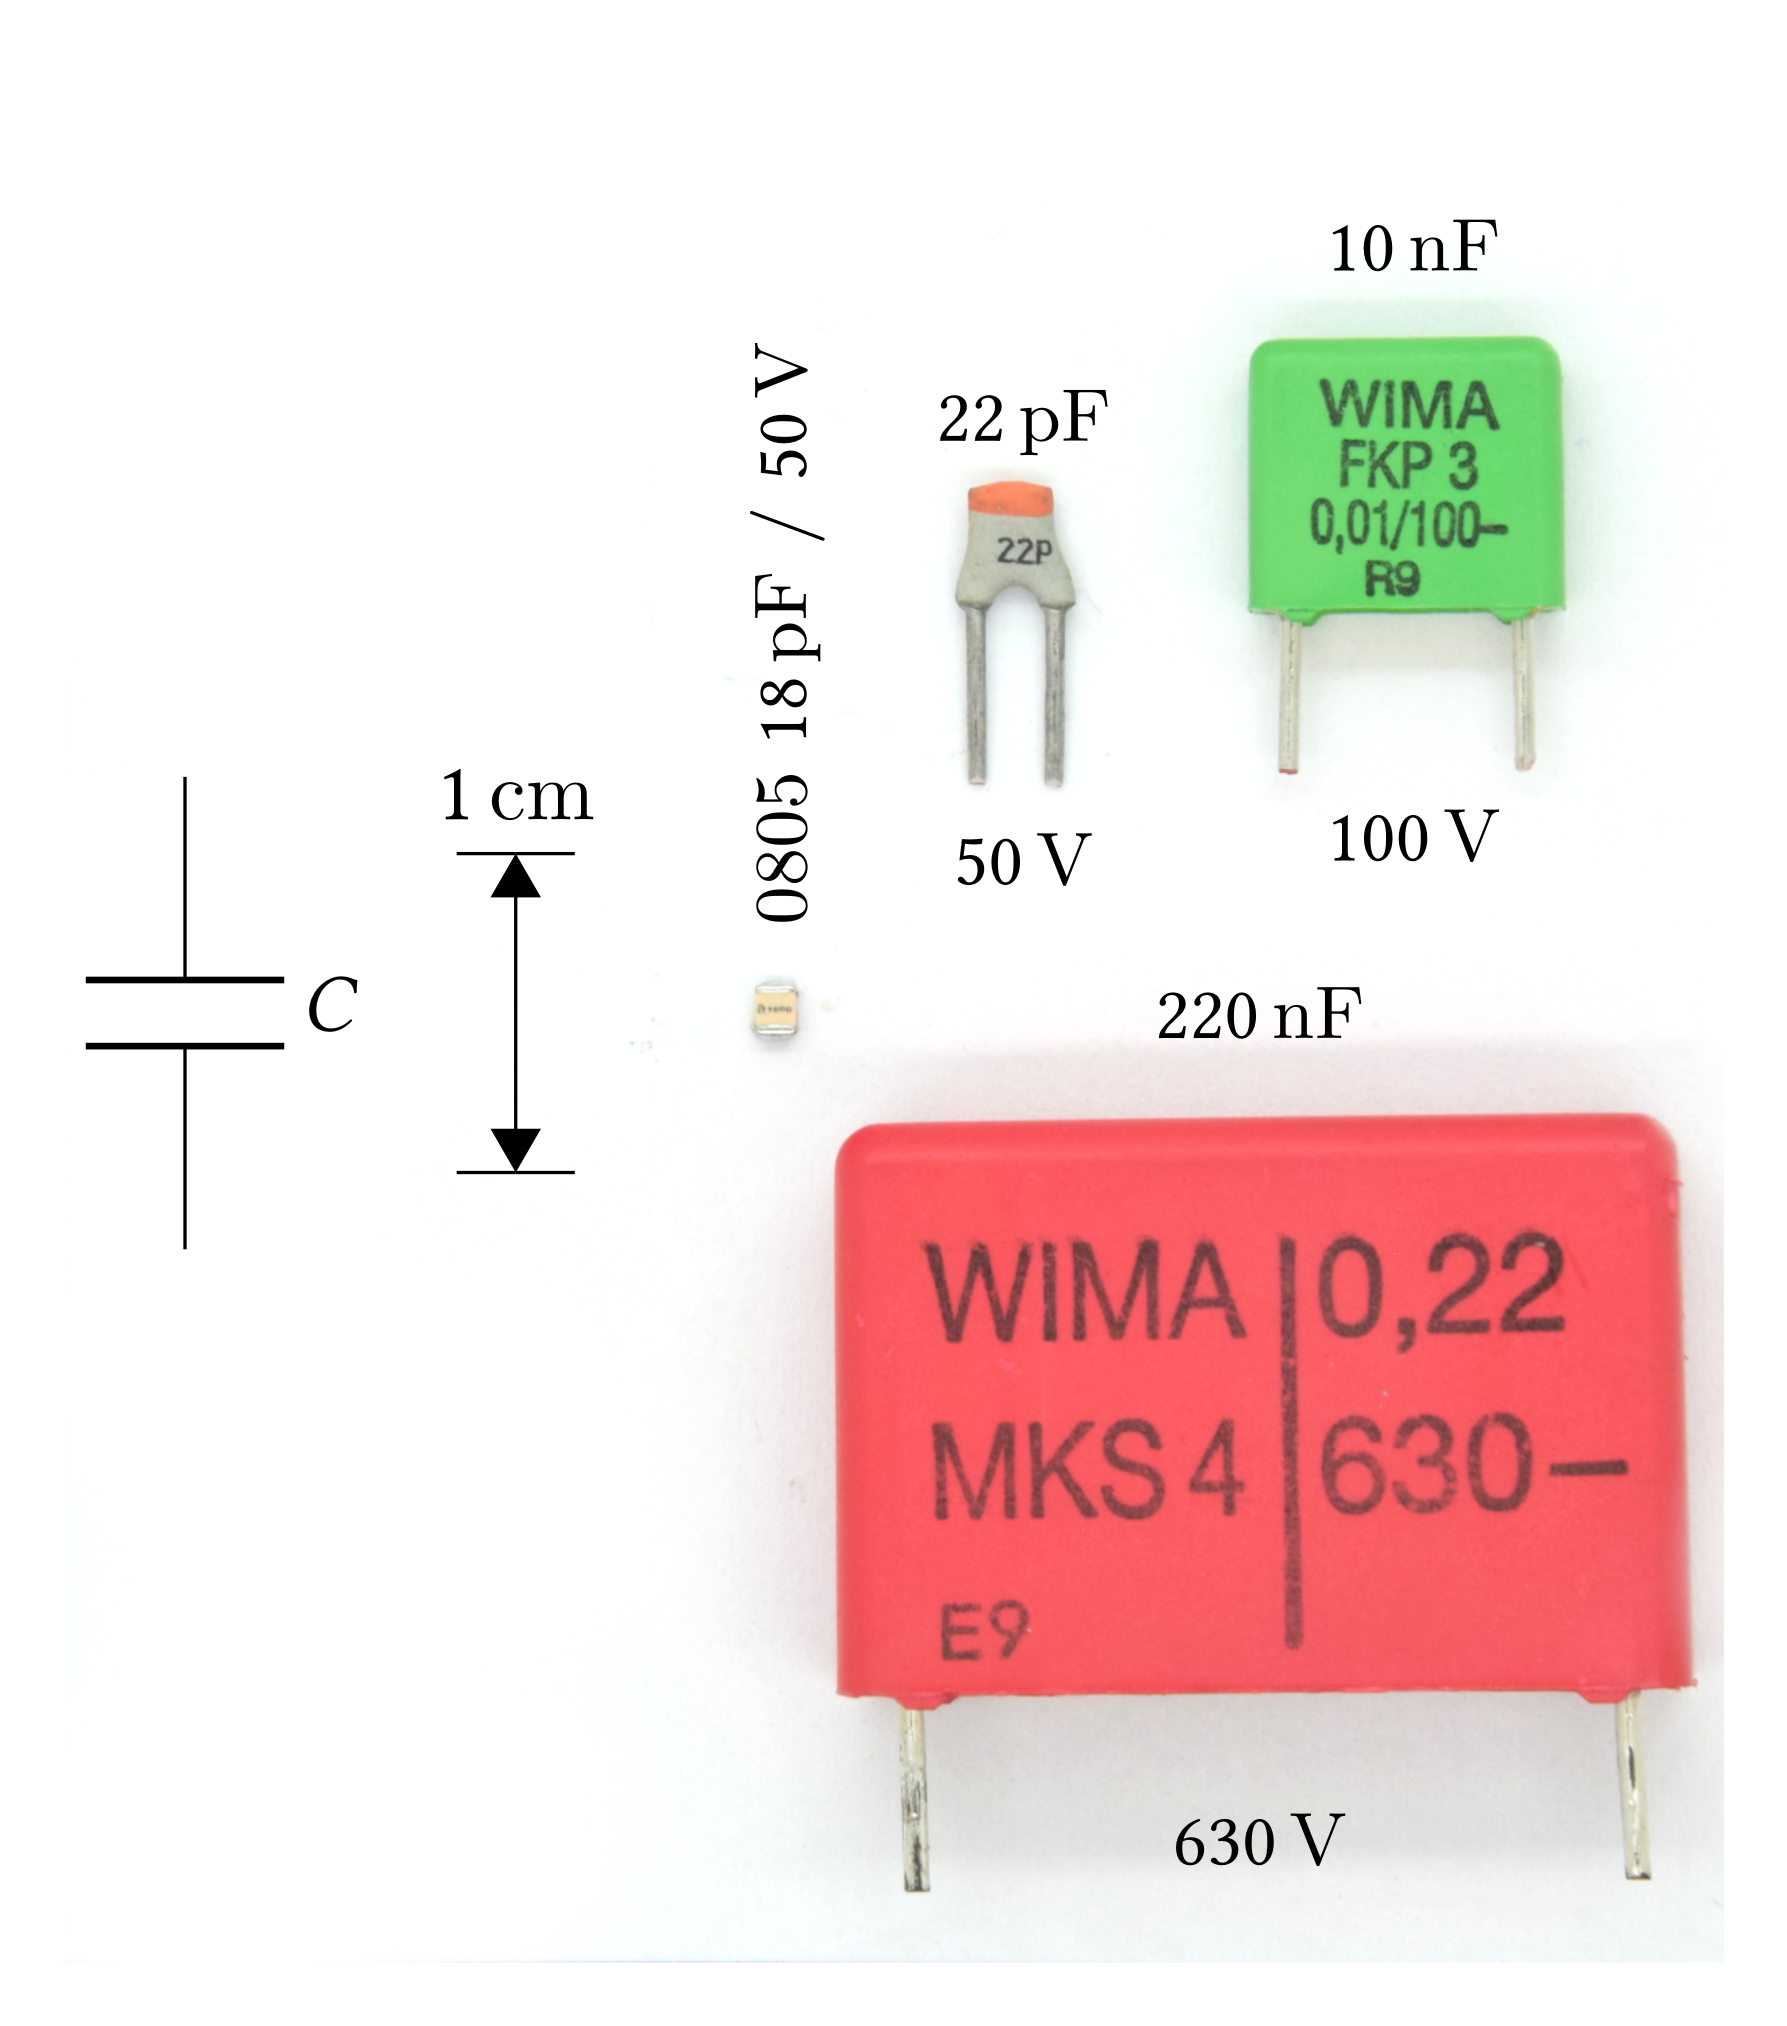
\includegraphics[width=0.85\textwidth]{foto/206}
    \caption{\scriptsize Schaltzeichen und Bauformen von Kondensatoren}
    \label{n_bauelemente_kondensator}
\end{figure}

   \end{column}
\end{columns}

\end{frame}

\begin{frame}
\only<1>{
\begin{PQuestion}{NC201}{Welches Bauteil wird durch das Schaltzeichen symbolisiert?}{Transistor}
{Spule}
{Kondensator}
{Batterie}
{\DARCimage{0.5\linewidth}{511include}}\end{PQuestion}

}
\only<2>{
\begin{PQuestion}{NC201}{Welches Bauteil wird durch das Schaltzeichen symbolisiert?}{Transistor}
{Spule}
{\textbf{\textcolor{DARCgreen}{Kondensator}}}
{Batterie}
{\DARCimage{0.5\linewidth}{511include}}\end{PQuestion}

}
\end{frame}

\begin{frame}
\frametitle{Spule}
\begin{columns}
    \begin{column}{0.48\textwidth}
    \begin{itemize}
  \item Speichert auch eine kleine Menge Energie
  \item Funktioniert technisch aber komplett anders als der Kondensator
  \item Besteht in den einfachen Fällen aus einem aufgewickelten Draht
  \end{itemize}

    \end{column}
   \begin{column}{0.48\textwidth}
       
\begin{figure}
    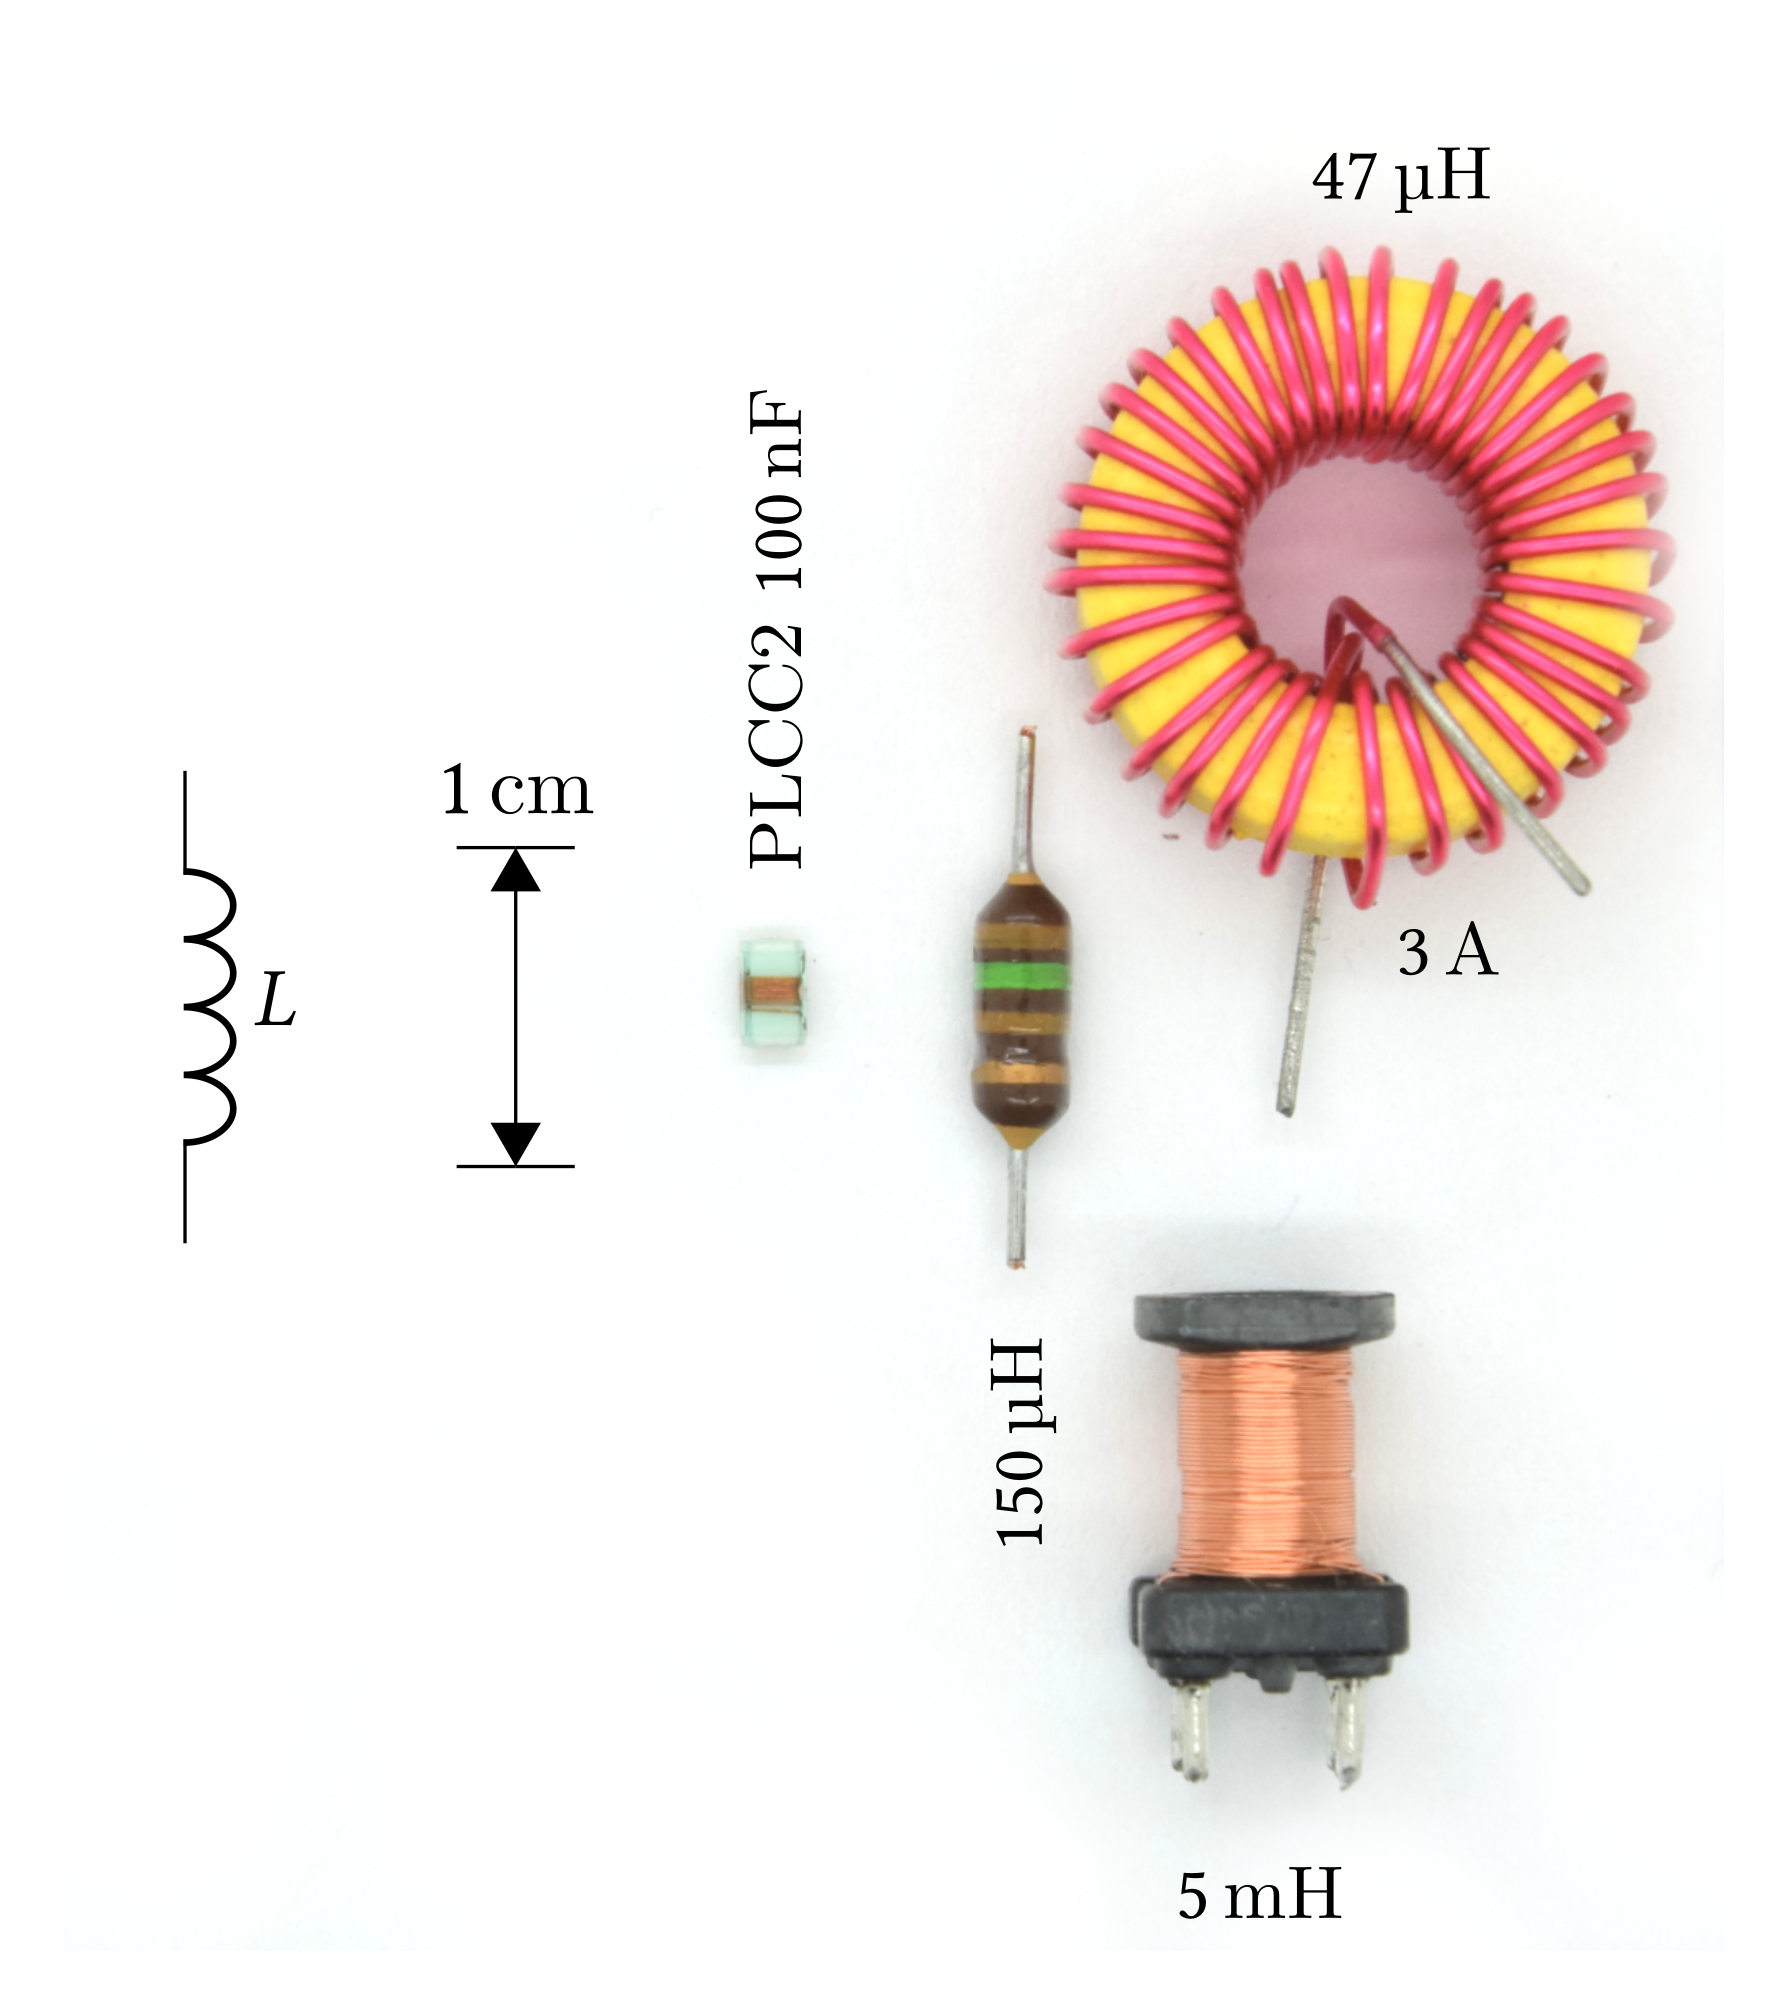
\includegraphics[width=0.85\textwidth]{foto/207}
    \caption{\scriptsize Schaltzeichen und Bauformen von Spulen}
    \label{n_bauelemente_spule}
\end{figure}

   \end{column}
\end{columns}

\end{frame}

\begin{frame}
\only<1>{
\begin{PQuestion}{NC301}{Welches Bauteil wird durch das Schaltzeichen symbolisiert?}{Diode}
{Kondensator}
{Spule}
{Batterie}
{\DARCimage{0.5\linewidth}{512include}}\end{PQuestion}

}
\only<2>{
\begin{PQuestion}{NC301}{Welches Bauteil wird durch das Schaltzeichen symbolisiert?}{Diode}
{Kondensator}
{\textbf{\textcolor{DARCgreen}{Spule}}}
{Batterie}
{\DARCimage{0.5\linewidth}{512include}}\end{PQuestion}

}
\end{frame}

\begin{frame}
\frametitle{Transistor}
\begin{columns}
    \begin{column}{0.48\textwidth}
    \begin{itemize}
  \item Elektrischer Schalter
  \item Oder Verstärker, je nach Beschaltung
  \item Hat drei Anschlüsse
  \end{itemize}

    \end{column}
   \begin{column}{0.48\textwidth}
       
\begin{figure}
    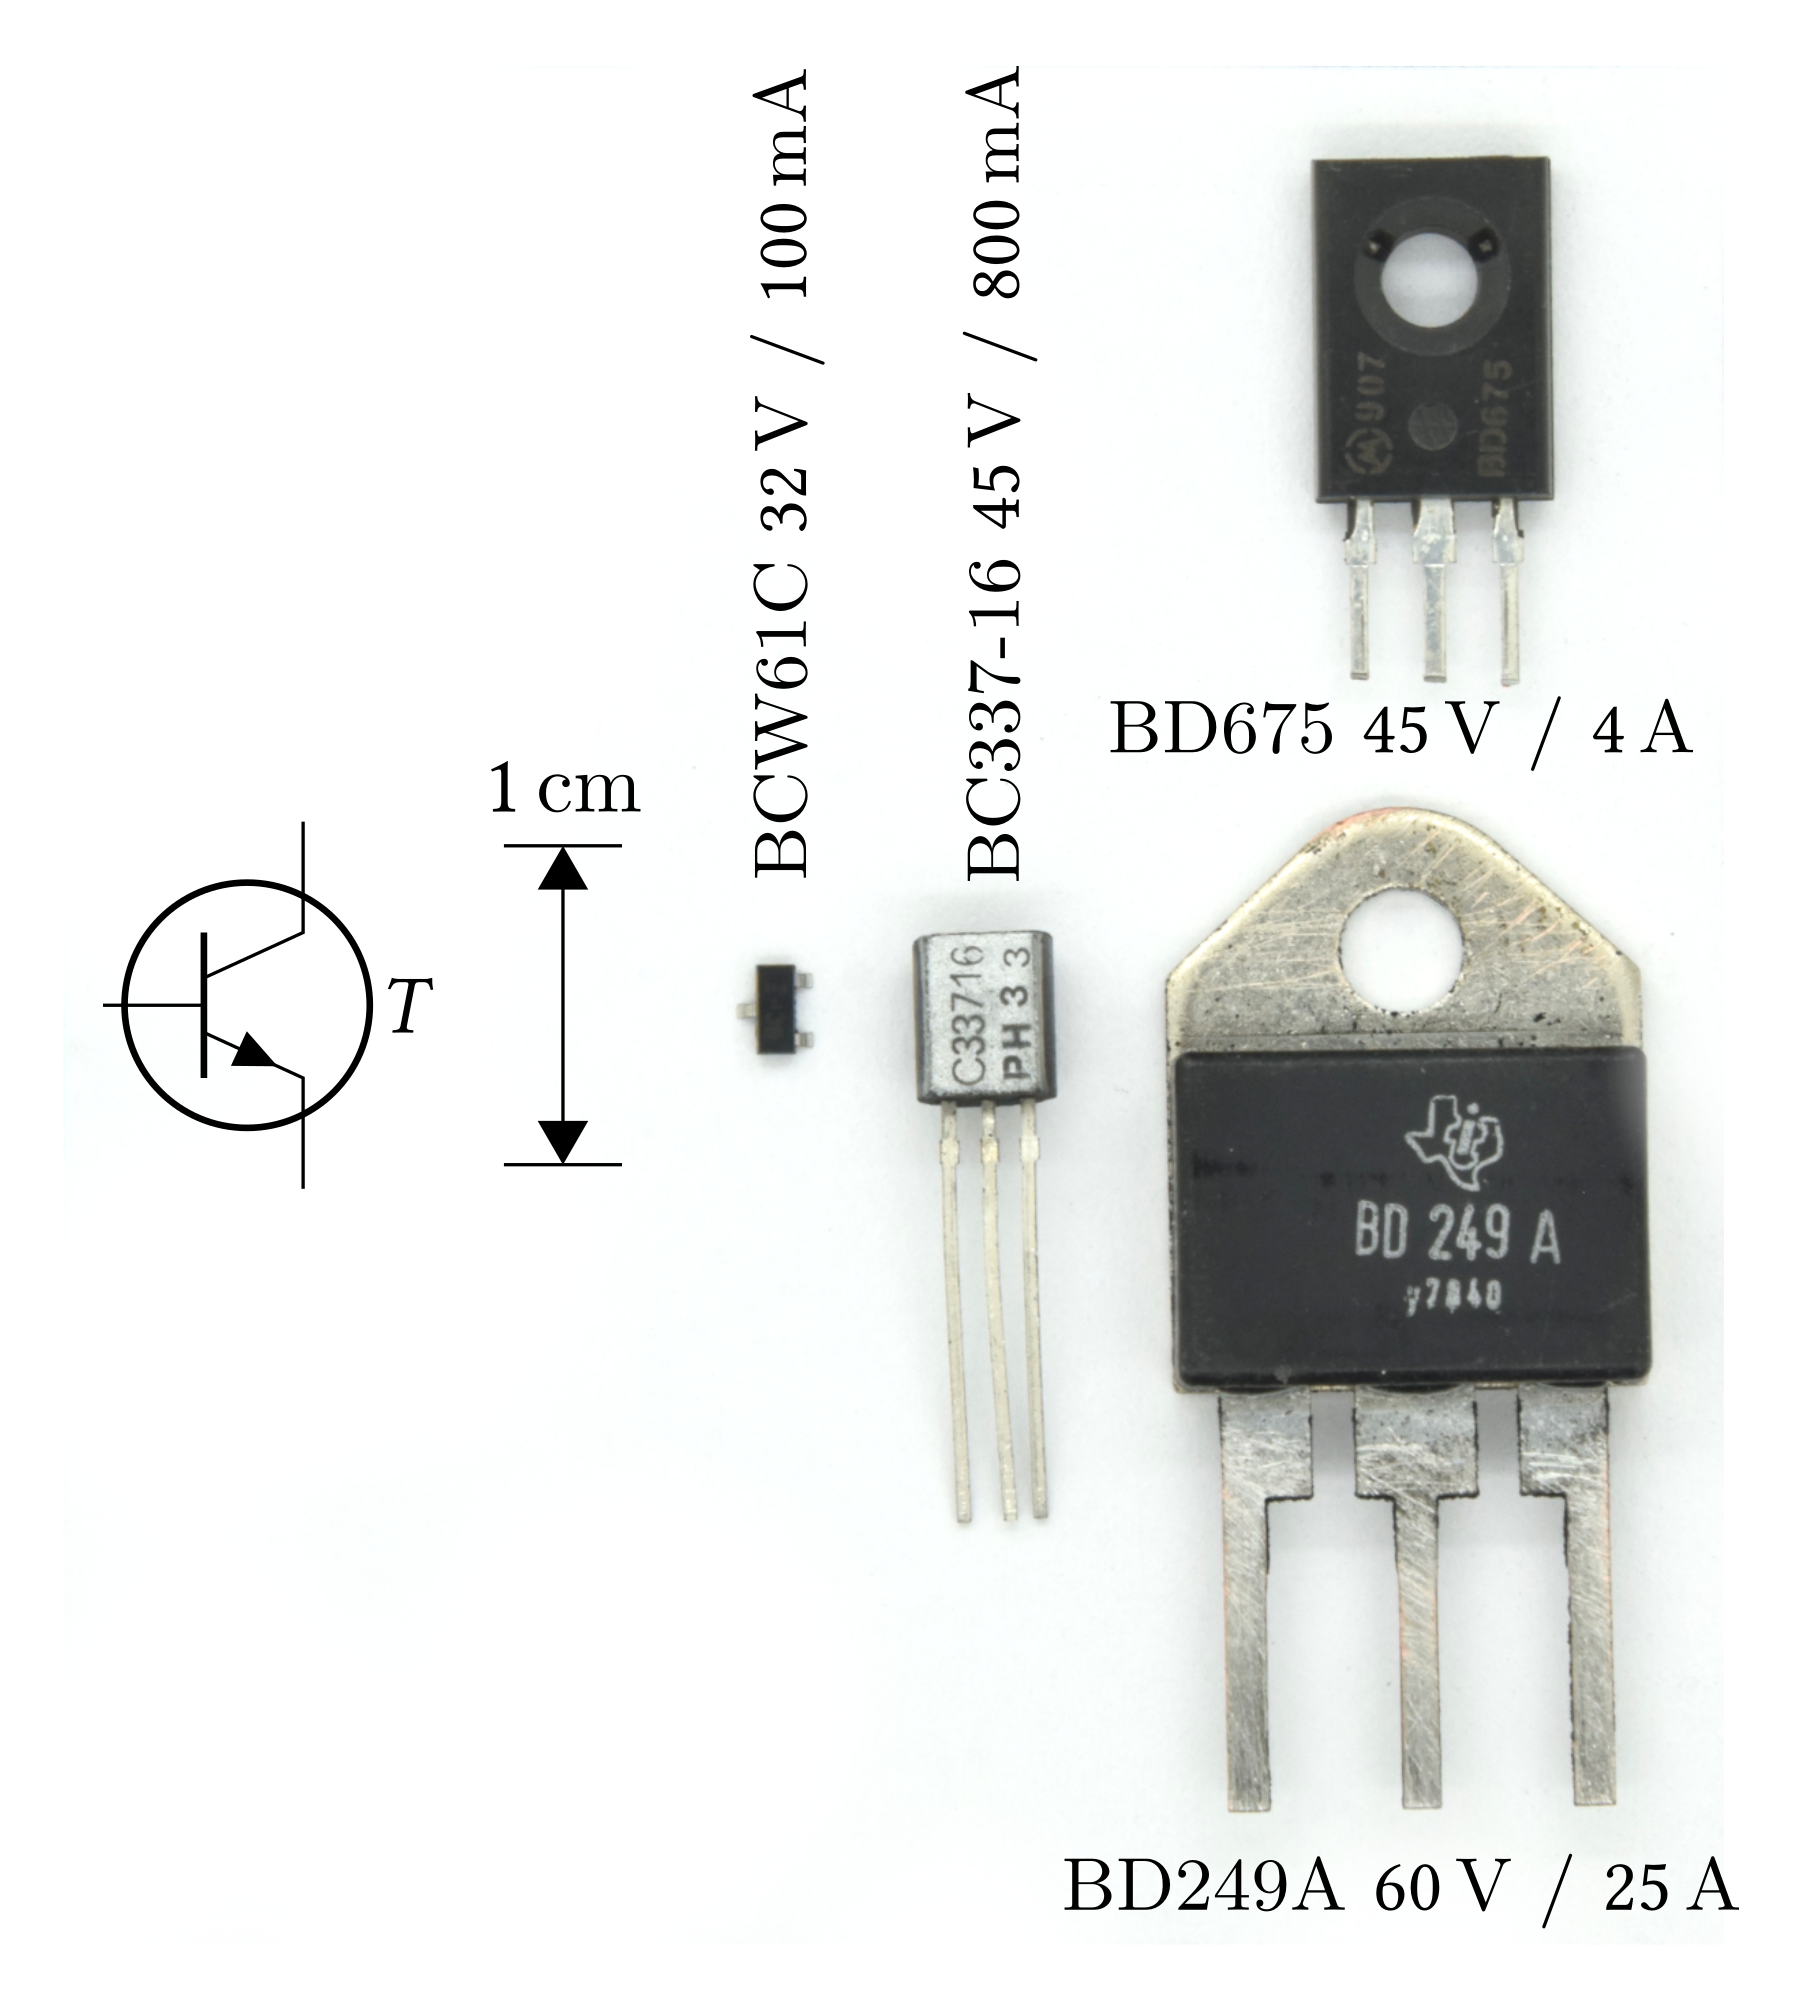
\includegraphics[width=0.85\textwidth]{foto/208}
    \caption{\scriptsize Schaltzeichen und Bauformen von Transistoren}
    \label{n_bauelemente_transistor}
\end{figure}

   \end{column}
\end{columns}

\end{frame}

\begin{frame}
\only<1>{
\begin{PQuestion}{NC501}{Welches Bauteil wird durch das Schaltzeichen symbolisiert?}{Diode}
{Spule}
{Kondensator}
{Transistor}
{\DARCimage{0.25\linewidth}{374include}}\end{PQuestion}

}
\only<2>{
\begin{PQuestion}{NC501}{Welches Bauteil wird durch das Schaltzeichen symbolisiert?}{Diode}
{Spule}
{Kondensator}
{\textbf{\textcolor{DARCgreen}{Transistor}}}
{\DARCimage{0.25\linewidth}{374include}}\end{PQuestion}

}
\end{frame}%ENDCONTENT
